%
% $RCSfile: approach.tex,v $
%
% Copyright (c) 2005-2006. Christian Heller. All rights reserved.
%
% Permission is granted to copy, distribute and/or modify this document
% under the terms of the GNU Free Documentation License, Version 1.1 or
% any later version published by the Free Software Foundation; with no
% Invariant Sections, with no Front-Cover Texts and with no Back-Cover
% Texts. A copy of the license is included in the section entitled
% "GNU Free Documentation License".
%
% http://www.cybop.net
% - Cybernetics Oriented Programming -
%
% http://www.resmedicinae.org
% - Information in Medicine -
%
% Version: $Revision: 1.1 $ $Date: 2006-01-03 08:21:45 $ $Author: christian $
% Authors: Christian Heller <christian.heller@tuxtax.de>
%

\section{Approach}
\label{approach_heading}

On its way to solving the issues mentioned in sections
\ref{introduction_heading} and \ref{architectural_troubles_heading}, the
work followed the \emph{Cybernetics Oriented Programming} (CYBOP) approach
\cite{heller2004}. The idea behind is as simple as it is helpful; it suggests
to:

\begin{center}
    Inspect solutions of various disciplines\\
    of science, phenomenons of nature,\\
    and apply them to software engineering.
\end{center}

Figure \ref{mindmap_figure} shows some sciences whose principles were
considered in this work. The name of a field of science is shown on top of each
box. Made observations are mentioned below, in the middle. The resulting design
recommendations for software can be found at the bottom of each box. The
recommendations are grouped into those that justify a distinction between
\emph{Statics and Dynamics}, a new kind of \emph{Knowledge Schema} and a
separation of \emph{State- and Logic} models.

\begin{figure}[ht]
    \begin{center}
        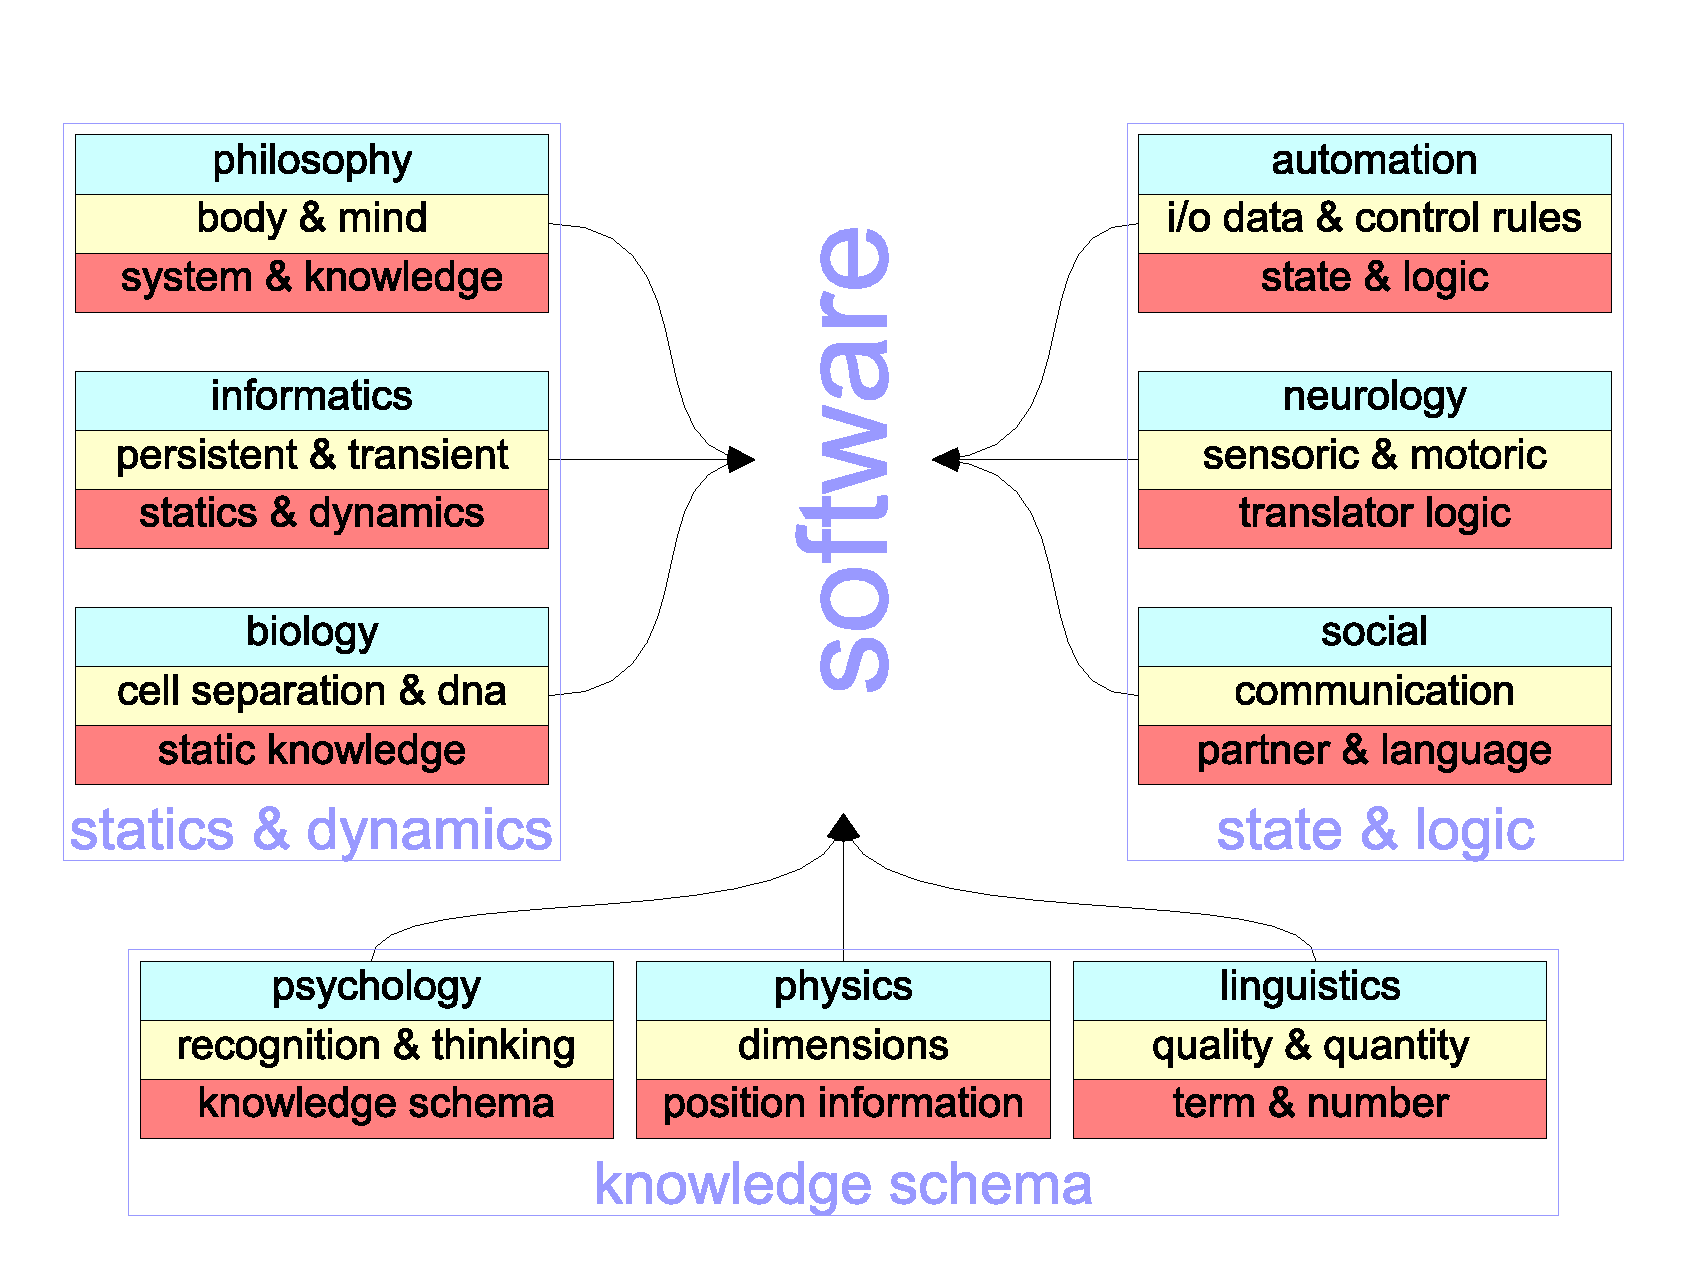
\includegraphics[scale=0.2]{vector/mindmap.eps}
        \caption{Mindmap of Influential Sciences}
        \label{mindmap_figure}
    \end{center}
\end{figure}

\begin{figure}[ht]
    \begin{center}
        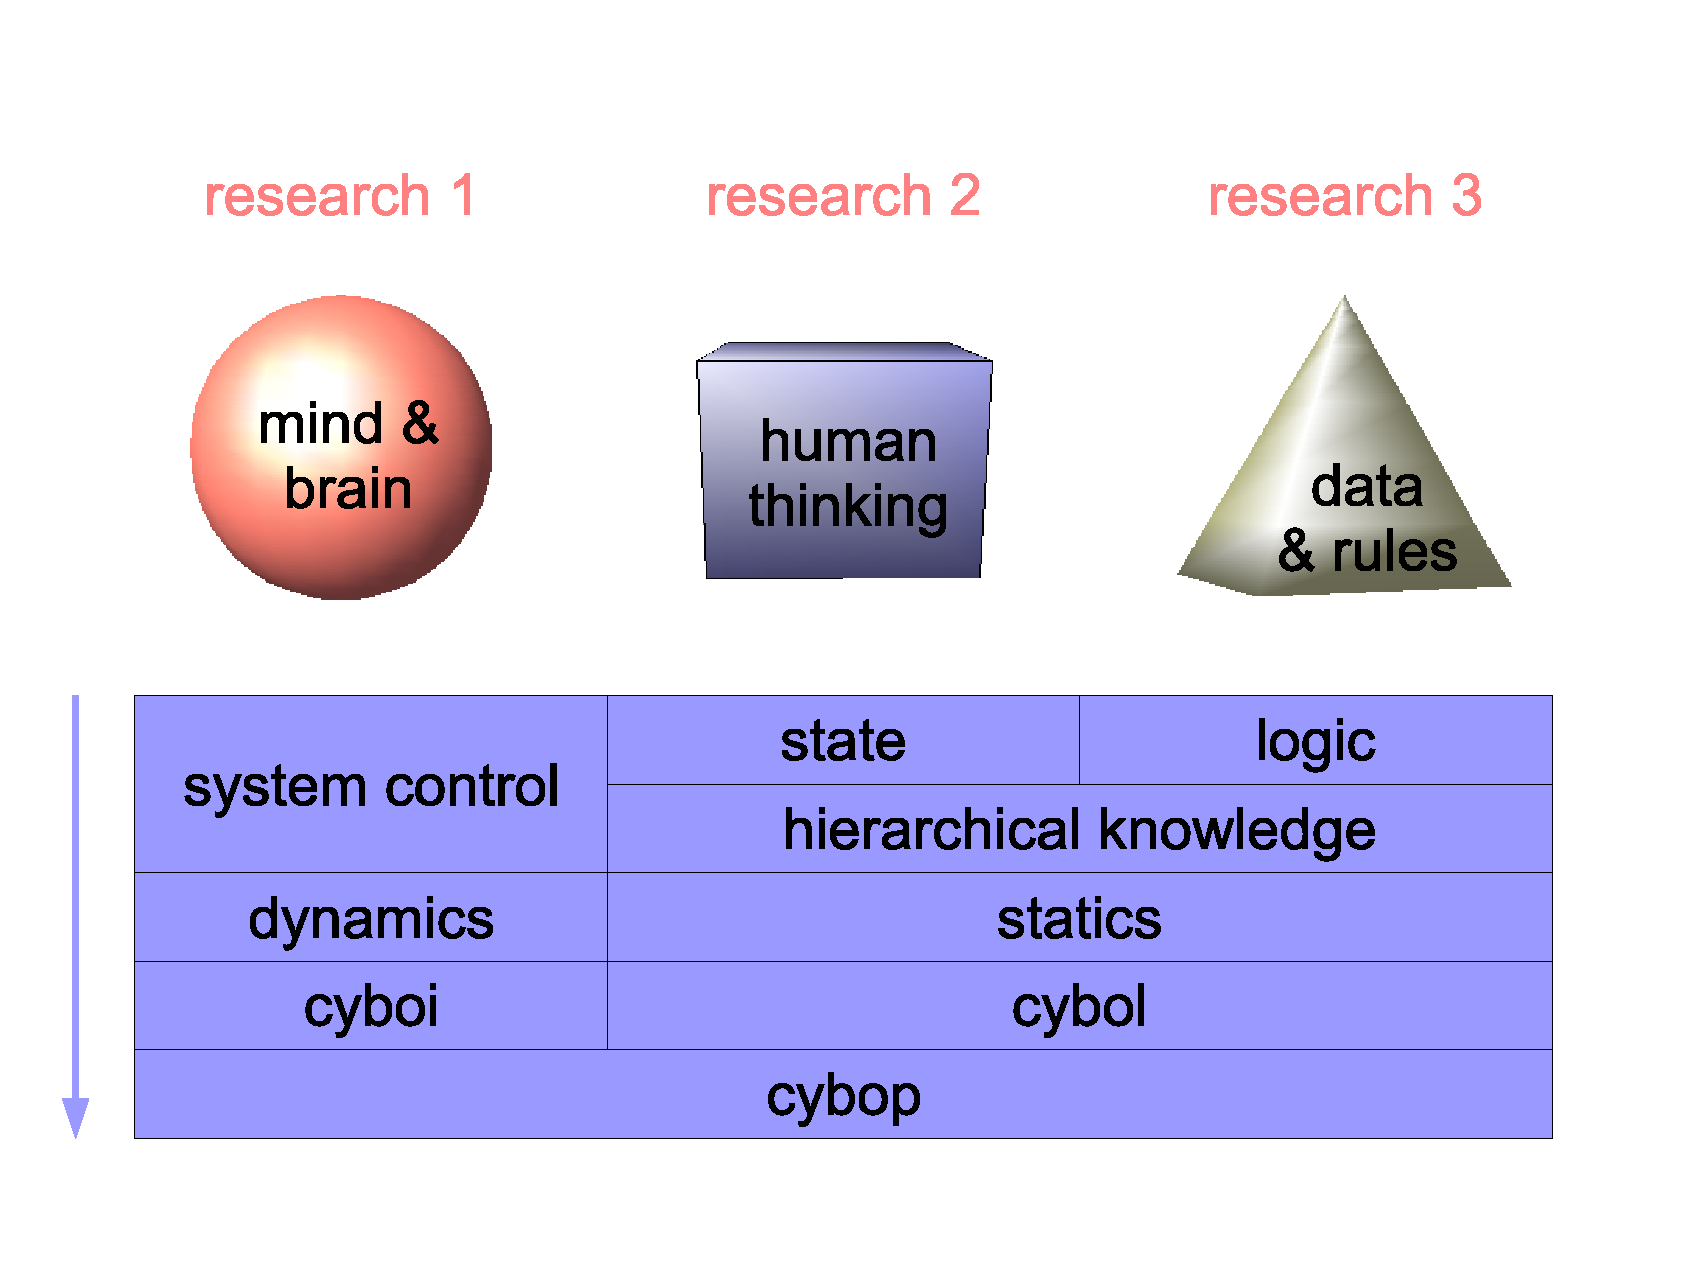
\includegraphics[scale=0.2]{vector/approach.eps}
        \caption{Overall CYBOP Approach}
        \label{approach_figure}
    \end{center}
\end{figure}

A first observation, when looking at human beings from a philosophical
perspective, is the separation of \emph{Mind} and \emph{Brain} (Body).
Accordingly, CYBOP treats computers as \emph{Systems} owning and processing
\emph{Knowledge}. This is not unlike the idea of \emph{Agent} systems owning a
\emph{Knowledge Base} \cite{parks, kuehnel}. All abstract knowledge that humans
make up belongs to their mind. The brain is merely a physical carrier of
knowledge. Similarly, there are actually two kinds of software: one
representing \emph{passive} knowledge and the other \emph{actively} controlling
a system's hardware.

Secondly, attention is payed to the concepts of \emph{Human Thinking}
\cite{heller2004}, as investigated by psychology. Through their application,
knowledge becomes \emph{hierarchical}. Moreover, this work tries to embed
knowledge models in an environment of \emph{Dimensions}, as known from physics.
Every model keeps a number of \emph{Meta Information} about its parts.
\emph{Positions} in space or time are one such example.

Thirdly, \emph{State-} gets distinguished from \emph{Logic} knowledge. It is
known from neurological research that the human brain has special communication
regions that, simply spoken, do nothing else than translating data, i.e. an
input- into an output \emph{State}, according to rules of \emph{Logic}. Systems
theory uses similar abstractions. When talking about states, this work means a
composed \emph{Set} of states.

In CYBOP (figure \ref{approach_figure}), all knowledge (states and logic),
belongs to a system's \emph{Statics}, and is described by CYBOL language
templates (section \ref{practical_proof_heading}). The processing of knowledge
at runtime, to control a system, is \emph{Dynamics} and happens in the CYBOI
interpreter.
